%%%%%%%%%%%%%%%%%%%%%%%%%%%%%%%%%%%%%%%%%%%%%%%%%%%%%%%%%%%%%%%%%%%%%%%%%%%%
% Nick Waters's super awesome template for bioRxiv and suppl submissions
% In memory of Henry, Hermione, and Angus.
% May there be many tasty snails in pufferfish heaven
%%%%%%%%%%%%%%%%%%%%%%%%%%%%%%%%%%%%%%%%%%%%%%%%%%%%%%%%%%%%%%%%%%%%%%%%%%%%
\documentclass[10pt]{article}
% \includeonly{supp_tex/figsgage}
\usepackage{geometry}
\geometry{marginparwidth=1cm,a4paper,verbose,tmargin=1.5cm,bmargin=1.5cm,lmargin=1.5cm,rmargin=1.5cm,headheight=0cm,headsep=0cm,footskip=0cm}
\usepackage{cite}
% \usepackage{ifthen}  % for plotting lots of figures in loops with conditionals
\usepackage{float}  % for forcing figures to stay put
\usepackage{hyperref} % make the references clickable
\setlength\parindent{0pt} % set indent to zero
\setlength{\parskip}{1.2em} % give a bit of space between paragraphs

\bibliographystyle{plain} % citation and bib style
\usepackage{grffile} %for underscores in file names
\usepackage{rotating} % for sideways tables
\usepackage[ruled]{algorithm2e} % for typesetting the riboSeed algorithm
\setlength{\algotitleheightrule}{0pt}
\usepackage{lineno, color} % controls line numbering
\modulolinenumbers[5]  % number every 5th line
% format our line numbers, cause no one likes boring numbers
\renewcommand\linenumberfont{\normalfont\tiny\color{blue}}
\usepackage{booktabs}  % less yucky tables
% nice little thing for table spacing (thanks Markus Püschel)
\newcommand{\ra}[1]{\renewcommand{\arraystretch}{#1}}
\usepackage{multirow} % for some pretty tables with merged cells
\usepackage[table,xcdraw]{xcolor} % for cool table cell colors
\usepackage{tikz}  % just so I can use \foreach
% my lined-off abstract
\newenvironment{myabstract}{%
\begin{quote} \baselineskip14pt \rule{.89\textwidth}{1.5pt} \vskip .1cm}
{ \vskip -.10cm \rule{.89\textwidth}{1.5pt} \end{quote}}

% supplementary (essentialy just resets numbering)
\newcommand{\beginsupplement}{%
  \setcounter{table}{0}
  \renewcommand{\thetable}{S\arabic{table}}%
  \setcounter{figure}{0}
  \renewcommand{\thefigure}{S\arabic{figure}}%
}
% pretty thought break
\def \thoughtbr {\begin{center}\noindent\rule{.4\textwidth}{0.4pt}  {\raisebox{-.5ex}{$\sim$}}  \rule{.4\textwidth}{0.4pt}\end{center}}

% \usepackage{graphicx}
\graphicspath{ {./riboFigs/} }  %  set the path to the figures

\usepackage{titlesec} % for adjusting spacing after the section headers
\titlespacing\subsection{0pt}{12pt plus 4pt minus 2pt}{-11pt plus 0pt minus 0pt}
\titlespacing\subsubsection{0pt}{12pt plus 4pt minus 2pt}{-11pt plus 0pt minus 0pt}


%%%%%%%%%%%%%%%%%%%%%%%%%%%%%%%%%%%%%%%%%%%%%%%%%%
% this hack stolen from Stack overflow is a macro to make a \cmmidrule
% for each column.  I added the ".4" spacing to get this to look prettier
%  if you have 5 columns, instead of \midrule, you could use \cmidrules{5}
\makeatletter
\newtoks\MD@cmidrules
\newcommand{\cmidrules}[1]{%
  \noalign{%
    \global\MD@cmidrules={}%
    \toks@={\cmidrule(l{.3\tabcolsep}r{.3\tabcolsep})}%
    \count@=\z@
    \loop\ifnum\count@<#1\relax
      \advance\count@\@ne
      \edef\MD@temp{\the\toks@{\the\count@-\the\count@}}%
      \global\MD@cmidrules\expandafter{\the\expandafter\MD@cmidrules\MD@temp}%
    \repeat
  }%
  \the\MD@cmidrules
}
\makeatother
%%%%%%%%%%%%%%%%%%%%%%%%%%%%%%%%%%%%%%%%%%%%%%%%%%

%%%%  This allows us to set the table font size up top
\usepackage{etoolbox}
\BeforeBeginEnvironment{tabular}{\begin{center}\footnotesize}
\AfterEndEnvironment{tabular}{\end{center}}
%%%%

\def \coli#1 {\textit{E.~coli~#1~}} %  #lazy
\def \ttilde {\raisebox{-.5ex}\textasciitilde} % fix for ugly cmodern tilde 20160829

%  format captions
\usepackage[%
    font={small},
    labelfont=bf,
    format=hang,
    format=plain,
    margin=0pt,
    width=0.9\textwidth]{caption}
\usepackage[list=true]{subcaption}  % allow for subfigures with captions
\usepackage{amssymb}  % for checkmark symbols
\usepackage{graphicx}  % trim figures
\usepackage{colortbl}  % adjust table colors
\definecolor{lgray}{gray}{.90}  % line grey
\definecolor{tgray}{gray}{.40}  % text grey
\definecolor{egray}{gray}{.01}  % emphasis grey
\usepackage[yyyymmdd,hhmmss]{datetime} % for timestamp

\title{\textbf{Supplementary Data}\\ \fontseries{m}\selectfont riboSeed: leveraging prokaryotic genomic architecture to assemble across ribosomal regions}

\author
{\small Nicholas R. Waters,$^{1,2}$ Florence Abram,$^{1}$ Fiona Brennan,$^{1,3}$ Ashleigh Holmes,$^{4}$ and Leighton Pritchard$^{2\ast}$\\
\\
\normalsize{\textit {$^{1}$Department of Microbiology, School of Natural Sciences, National University of Ireland, Galway, Ireland}}\\
\normalsize{\textit {$^{2}$Information and Computational Sciences, James Hutton Institute, Invergowrie, Dundee DD2 5DA, Scotland}}\\
\normalsize{\textit {$^{3}$Soil and Environmental Microbiology, Environmental Research Centre, Teagasc, Johnstown Castle, Wexford, Ireland}}\\
\normalsize{\textit {$^{4}$Cell and Molecular Sciences, James Hutton Institute, Invergowrie, Dundee DD2 5DA, Scotland}}\\
\\
\footnotesize{$^\ast$To whom correspondence should be addressed: leighton.pritchard@hutton.ac.uk}
}
\date{}

\begin{document}
\baselineskip20pt  % set line spacing; double spacing is 2xfontsize, in this case 11
\maketitle
\vspace*{-1.5cm}
{\begin{center}\footnotesize\date{Compiled: \today ~\currenttime}\end{center}}


\beginsupplement

\section*{Extended Methods}

\subsection*{Reference Selection Recommendations}
Using a recently-diverged reference sequence maximizes chances of a successful assembly. We have outlined two methods to select an appropriate reference for a given isolate: a robust method using Kraken, and a quick method using Reads2Type.

\subsubsection*{Method 1: Kraken}

Kraken \cite{Wood2014} is a \textit{k}-mer-based phylogeny tool that can be used to identify the strains present in a metagenomic dataset; installation and usage instructions can be found here: \href{https://ccb.jhu.edu/software/kraken/}{https://ccb.jhu.edu/software/kraken/}. After downloading and installing Kraken, along with the MiniKraken database from their website, Kraken can be run on an isolate's reads, generating the a taxonomy report.

The MiniKraken database was built from all the complete genomes from RefSeq, allowing the user to identify which strain in the database has the closest match to the sequenced isolate.

\subsubsection*{Method 2: Reads2Type and  cgFind}
Reads2Type \cite{Saputra2015} is also a \textit{k}-mer-based phylogeny tool, but it relies on a lightweight, prebuilt database of 55-mers from a set of reference strains. This allows the analysis to be performed in the web browser, and it does not require the user to upload complete read files, allowing it to perform well when either speed or network access is limited.  It works by taking one read at a time from the input file, generating 55-mers, and comparing to a prebuilt database. If there is not enough resolution information to identify the isolate by that read alone, additional reads are processed until a single taxonomy identification is achieved.  This method works best on trimmed reads. Instructions and the webserver can be found at \href{https://cge.cbs.dtu.dk/services/Reads2Type/}{https://cge.cbs.dtu.dk/services/Reads2Type/}

Given the genus and species from Reads2Type, users can make use of cgFind, a web tool we developed to provide easy access to downloadable genomes based on the complete prokaryotic genomes found in NCBI. The tool can be found at \href{https://nickp60.github.io/cgfind}{https://nickp60.github.io/cgfind}.


\subsection*{Making the artificial chromosome}
The artificial chromosome used for testing was constructed using the \texttt{makeToyGenome.sh} script included in the GitHub repository (\url{https://github.com/nickp60/riboSeed}) under the \textbf{\texttt{scripts}} directory. Briefly, the 7 rDNA regions from the \coli{Sakai} genome were extracted with 5kb flanking sequence upstream and downstream; these sequences were then concatenated end to end to form a single, $approx$100kb sequence containing the 7 rDNAs as well as their flanking context.


\subsection*{Effect of reference sequence identity on riboSeed performance}
The following range of substitutions were introduced into a artificial genome using the \texttt{runDegenerate.sh} script (included in the GitHub repository under the \textbf{\texttt{scripts}} directory), which facilitates the following procedure: 0.0, 0.0025, 0.0050, 0.0075, 0.0100, 0.0150, 0.0200, 0.0250, 0.0500, 0.0750, 0.1000, 0.1250, 0.1500, 0.1750, 0.2000, 0.2250, 0.2500, 0.2750, 0.3000. An artificial test genome is constructed (see above), and reads simulated using pIRS (100bp, 300bp inserts, stdev 10, 30-fold coverage, built-in error profile).  Then, for each of a range of substitution frequencies, substitutions are introduced into the simulated genome, either just in the flanking regions or uniformly throughout. riboSeed is run on the reads using the mutated genome as the reference, and the results are evaluated with riboScore. This script was run 100 times, using a different random seed each time.  As pseudo random number generation may differ between operating systems, comparable but not identical results can be expected.

\section*{Performance Across Prokaryotic Phyla}
\subsection*{Performance on Archaeal Data}

We assessed the effectiveness of riboSeed in assembling archaeal genomes. Most (\ttilde55\%) archaeal genomes have only a single rDNA, and none has been observed to have more than four. As riboSeed requires a sequencing dataset and a reference genome, our ability to benchmark was limited; of the 104 entries in \textit{rrn}DB with multiple rDNAs, only 7 had multiple entries at the species level. Among those, only 2 had publicly available short read data. We used riboSeed to re-assemble \textit{Methanosarcina barkeri Fusaro DSMZ804} (SRR2064286) and \textit{Methanobacterium formicicum st. JCM10132} (DRR017790).\textit{Methanosarcina barkeri Fusaro DSMZ804} and  \textit{Methanobacterium formicicum st. BRM9}  were the only ones that were suitable for riboSeed, in that there was publicly available short read data, more than a single rDNA operon, and an appropriate complete reference genome at the species level.  Results are shown in Table \ref{table:phyla}.

\textit{Methanosarcina barkeri Fusaro DSMZ804} was sequenced using an Illumina HiSeq2000 with 101bp paired-end reads, with an average fragment length of 400bp. We downsampled to use 5\% of the 19.4Gbp dataset with seqtk (\href{https://github.com/lh3/seqtk}{https://github.com/lh3/seqtk}). \textit{Methanosarcina barkeri str. Wiesmoor} (CP009526.1) was used as a reference. The resulting riboSeed assembly showed correct assembly of 3 of 3 rDNAs, while \textit{de novo} assemble failed to resolve any.

\textit{M. formicicum st. JCM10132} was sequenced on an Ion Torrent PGM, generating 106.5Mbp of 89bp single-end reads. \textit{M formicicum BRM9} (CP006933.1) was used as a reference. While riboSeed with default parameters did not resolve any of the assembly gaps (final assembly \textit{k}-mers 21, 33, 55, and 77), re-running the final assembly with \textit{k}-mers of 21, 33, 55, 77, and 99 resulted in closing 2 of 2 rDNA gaps. We are unsure why the addition of 99-mers improved assembly with 89-bp reads, but we are actively investigating this. This represents the first application of riboSeed to Ion Torrent data.

Taken together, we show that given appropriate datasets and parameters, archaeal datasets can be processed in the same manner used for bacteria.

\subsection*{Performance Across Bacterial Phyla}
In order to assess riboSeed's wider applicability, we selected additional datasets representing major bacterial phyla for those not already present in our analysis. In all cases, riboSeed improved the assemblies compared to the \textit{de novo} with no missassemblies introduced (Table \ref{table:phyla}). Thus, riboSeed can be applied to a wide range of organisms.

\begin{sidewaystable}[!hb]
  \centering
  \caption{Comparison of \textit{de novo} and riboSeed's \textit{de fere novo} assemblies}
  \label{table:phyla}
  %                 p       o         strain SRA       name     acc    rDNAs             good   -     bad            good    -      bad
  \begin{tabular}{p{2.25cm}p{2.65cm}p{5.75cm}p{1.75cm}p{2.25cm}p{1.95cm}p{.6cm}>{\hfill}p{.4cm}p{.2cm}p{.1cm}>{\hfill}p{.4cm}p{.2cm}p{.1cm}}
    % \arrayrulecolor{black}
    \toprule
    \multirow{2}{*}{Phylum} & \multirow{2}{*}{Class}  & \multicolumn{2}{l}{\textbf{Sequenced Strain}}  &  \multicolumn{3}{l}{\textbf{Reference Strain}} &  \multicolumn{3}{c}{\textit{de novo}} & \multicolumn{3}{c}{\textit{de fere novo}} \\
    & & Name & SRA & Name & Accession & rDNAs & \textbf{$\checkmark$} & -- & $\times$ & \textbf{$\checkmark$} & -- & $\times$  \\
   % \cmidrule{1-1}\cmidrule(l){2-2}\cmidrule(l){3-3}\cmidrule(l){4-4}\cmidrule(l){5-6}\cmidrule(l){7-9}\cmidrule(l){10-12}
    \toprule
    Actinobacteria & Actinobacteria        & \textit{Corynebacterium  diphtheriae}   NCTC 13129      & SRR4271515 & 241 &  NC\_016782.1      & 5  & \textbf{0} & 5  & 0 & \textbf{3} & 2 & 0 \\
    Chlamydiae     & Chlamydiia            & \textit{Chlamydia        trachomatis}  Population 1 & SRR5942978 & 434/Bu & NC\_010287.1     & 2  & \textbf{0} & 2  & 0 & \textbf{2} & 0 & 0 \\
    Firmicutes     & Clostridia            & \textit{Clostridioides   difficile}    C00005970                                             & ERR251735  & 630  &AM180355.1       & 11 & \textbf{0} & 11 & 0 & \textbf{9} & 2 & 0 \\
    Proteobacteria & Betaproteobacteria    & \textit{Burkholderia     cepacia}      DHQP2016-12-119                                       & SRR6334321 & ATCC25416       & NZ\_CP012981.1    & 6  & \textbf{0} & 6  & 0 & \textbf{3} & 3 & 0 \\
    Proteobacteria & Deltaproteobacteria   & \textit{Myxococcus       xanthus}      DSM 16526                                             & SRR4236978 & DK\_1622 & NC\_008095.1
  & 4  & \textbf{0} & 4  & 0 & \textbf{4} & 0 & 0 \\
    Proteobacteria & Epsilonproteobacteria & \textit{Helicobacter     cinaedi}      MRY12-0051                                            & DRR090193  & ATCC BAA-847 & NC\_020555.1 & 3  & \textbf{0} & 3  & 0 & \textbf{3} & 0 & 0 \\
    Tenericutes    & Mollicutes            & \textit{Mycoplasma       hominis}      Australia                                             & ERR1938252 & ATCC\_23114  &NC\_013511.1       & 2  & \textbf{0} & 2  & 0 & \textbf{2} & 0 & 0 \\
    Euryarchaeota  & Methanobacteria       & \textit{Methanobacterium formicicum}   JCM10132                                              & DRR017790  & BRM9        &CP006933.1        & 3  & \textbf{0} & 3  & 0 & \textbf{3} & 0 & 0 \\
    Euryarchaeota  & Methanomicrobia       & \textit{Methanosarcina    barkeri}     Fusaro DSMZ804                                        & SRR2064286 & Wiesmoor    &CP009526.1        & 2  & \textbf{0} & 2  & 0 & \textbf{2} & 0 & 0 \\
    % \arrayrulecolor{black}

    \bottomrule
    \begin{minipage}[t]{.5\textwidth}
      {\tiny
        $\checkmark$  correct assembly; --  unnassembled; $\times$  incorrect assembly\\
        % * run with \texttt{--centers 7:0} option to group tandem rDNAs
      }
    \end{minipage}
  \end{tabular}
\end{sidewaystable}



%  I need to do this to deal with the page breaks
\begin{figure}[]
  \centering
  \foreach \x in {1,2,...,5}{
    \begin{subfigure}[b]{.45\textwidth}
      \includegraphics[width=0.95\textwidth]{entropy_results_figs/\x_genome.png}
    \caption{}
    \end{subfigure}
    \begin{subfigure}[b]{.45\textwidth}
      \includegraphics[width=0.95\textwidth]{entropy_results_figs/\x_gene.png}
    \caption{}
    \end{subfigure}
  }
  \label{fig:ent_gage}
\end{figure}

% And each set here after
\begin{figure}[]\ContinuedFloat
  \centering
  \foreach \x in {6,7,...,10}
  {
    \begin{subfigure}[b]{.45\textwidth}
      \includegraphics[width=0.95\textwidth]{entropy_results_figs/\x_genome.png}
    \caption{}
    \end{subfigure}
    \begin{subfigure}[b]{.45\textwidth}
      \includegraphics[width=0.95\textwidth]{entropy_results_figs/\x_gene.png}
    \caption{}
    \end{subfigure}
  }
\end{figure}

% 11-15
% 12 Sakai was omitted, as it was present in manuscript
\begin{figure}[]\ContinuedFloat
  \centering
  \foreach \x in {11,12,13,15}
  {
    \begin{subfigure}[b]{.45\textwidth}
      \includegraphics[width=0.95\textwidth]{entropy_results_figs/\x_genome.png}
    \caption{}
    \end{subfigure}
    \begin{subfigure}[b]{.45\textwidth}
      \includegraphics[width=0.95\textwidth]{entropy_results_figs/\x_gene.png}
    \caption{}
    \end{subfigure}
  }
\end{figure}

% And each set here after
% 16 was omitted (duplicate P aeruginosa)
\begin{figure}[]\ContinuedFloat
  \centering
  \foreach \x in {17,...,21}
  {
    \begin{subfigure}[b]{.45\textwidth}
      \includegraphics[width=0.95\textwidth]{entropy_results_figs/\x_genome.png}
    \caption{}
    \end{subfigure}
    \begin{subfigure}[b]{.45\textwidth}
      \includegraphics[width=0.95\textwidth]{entropy_results_figs/\x_gene.png}
    \caption{}
    \end{subfigure}
  }
\end{figure}

%  I need to do this to deal with the page breaks
\begin{figure}[]\ContinuedFloat
  \centering
  \foreach \x in {21,22}{
    \begin{subfigure}[b]{.45\textwidth}
      \includegraphics[width=0.95\textwidth]{entropy_results_figs/\x_genome.png}
    \caption{}
    \end{subfigure}
    \begin{subfigure}[b]{.45\textwidth}
      \includegraphics[width=0.95\textwidth]{entropy_results_figs/\x_gene.png}
    \caption{}
    \end{subfigure}
  }
  \label{fig:ent_gage}
  \caption{riboScan.py, riboSelect.py, and riboSnag.py were run on all the genomes used as references for \textit{de fere novo} assemblies. Consensus alignment depth (grey bars) and Shannon entropy (black points, smoothed entropy as red line) for aligned rDNA regions.  Similar to Figure 3 in the main text, for each genome, a gene neighboring the first rDNA operon was identified, and used to extract homologous rDNA operons from up to 25 other isolates at the species level. In most cases, the entropy is lower in homologous rDNAs than across all the rDNAs in a given genome.  For strains with a low number of complete genomes for comparison available, entropy may be artificially increased (see \textit{Mycoplasma hominis}) or decreased (\textit{Helicobacter cinaedi}). A baseline entropy of greater than 0 may indicate equal distribution of two alleles of the operon either within a genome or across genomes.}
\end{figure}

\section*{Atypical rDNA operon structure}

Bacterial (and many archaeal) ribosomal RNA coding regions are commonly arranged into operons consisting of a 16S rRNA, 23S rRNA, and one or more 5S rRNAs, often with various tRNAs interspersed. In the course of this study, we observed some taxa lacking this typical 16S--23S--5S rRNA operon. When rDNAs are not structured into operons, assemblies from short reads do not suffer from the issue of long repeats and so do not require specialised approaches to assembly, such as riboSeed. We developed a module called \texttt{structure} for plotting rDNAs across a collection of genomes; this is available for riboSeed as of version 0.4.50.  Figure \ref{fig:atypical} show the operon arrangement of a few examples of organisms exhibiting atypical operon structure. For comparison, the rDNAs in the reference strains used in this study are shown in Figure \ref{fig:typical}.

\begin{figure}[H]
  \centering
  \hspace*{0cm}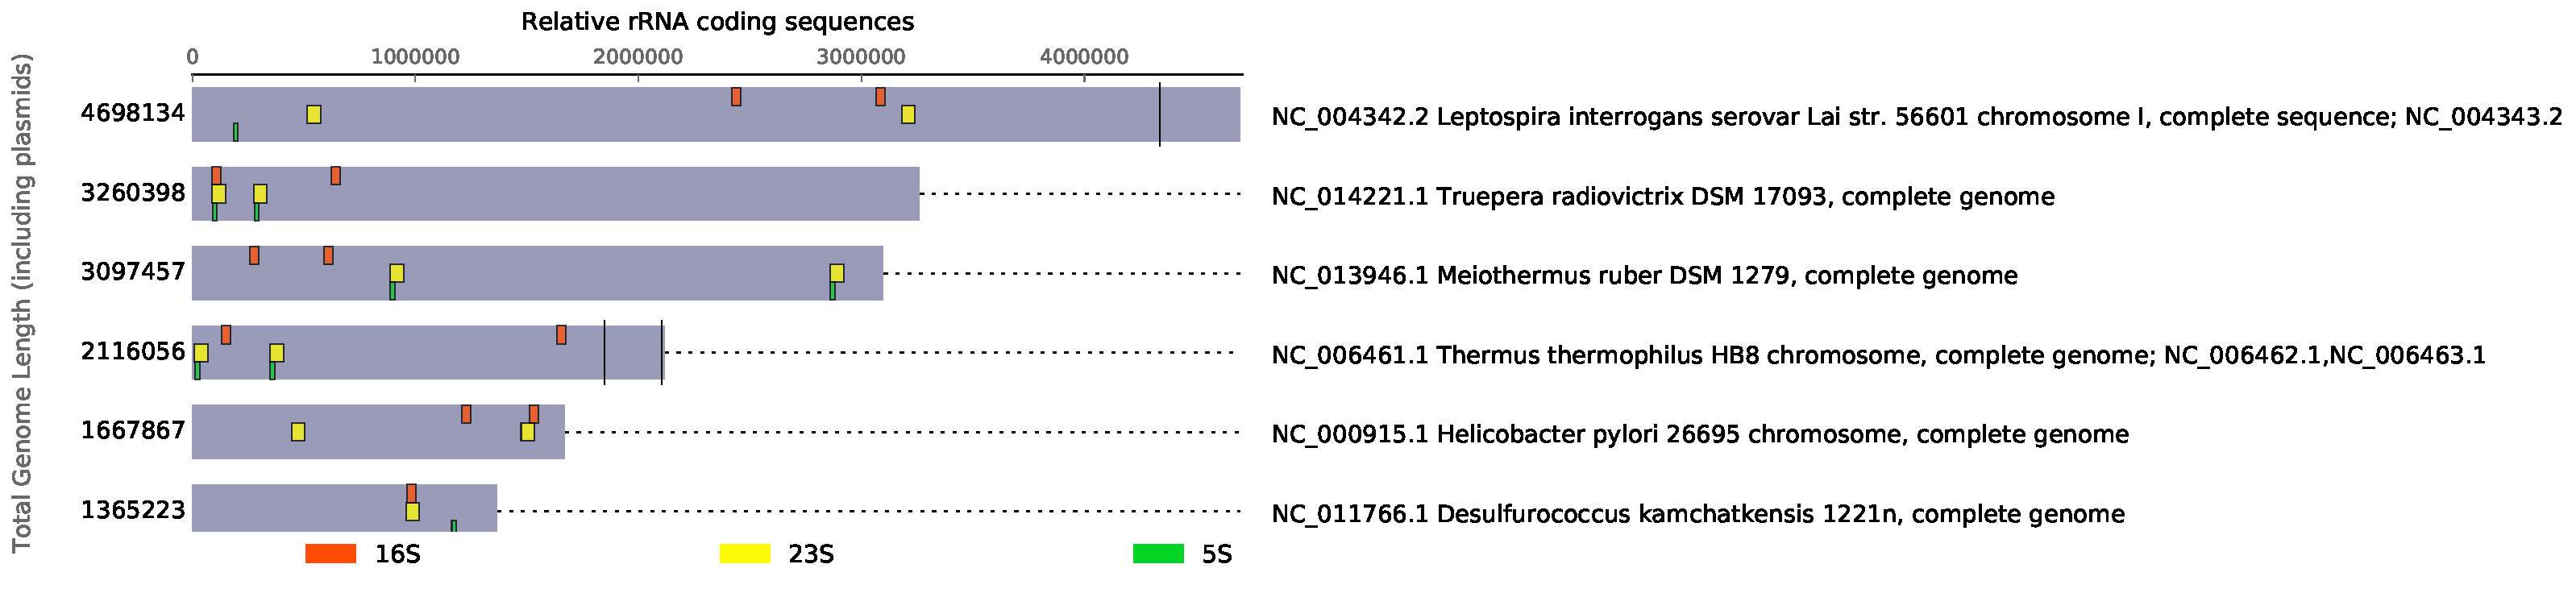
\includegraphics[width=1.0\textwidth]{odd_rDNA_relative_locations}
  \caption{Atypical rDNA operon structure in select taxa. rRNA lengths are not shown to scale. Note that the NCBI record for \textit{Helicobacter pylori} (NC\_000915.1) shows a 5S rRNA not detected by Barrnap. }
  \label{fig:atypical}
\end{figure}

\begin{figure}[H]
  \centering
  \hspace*{0cm}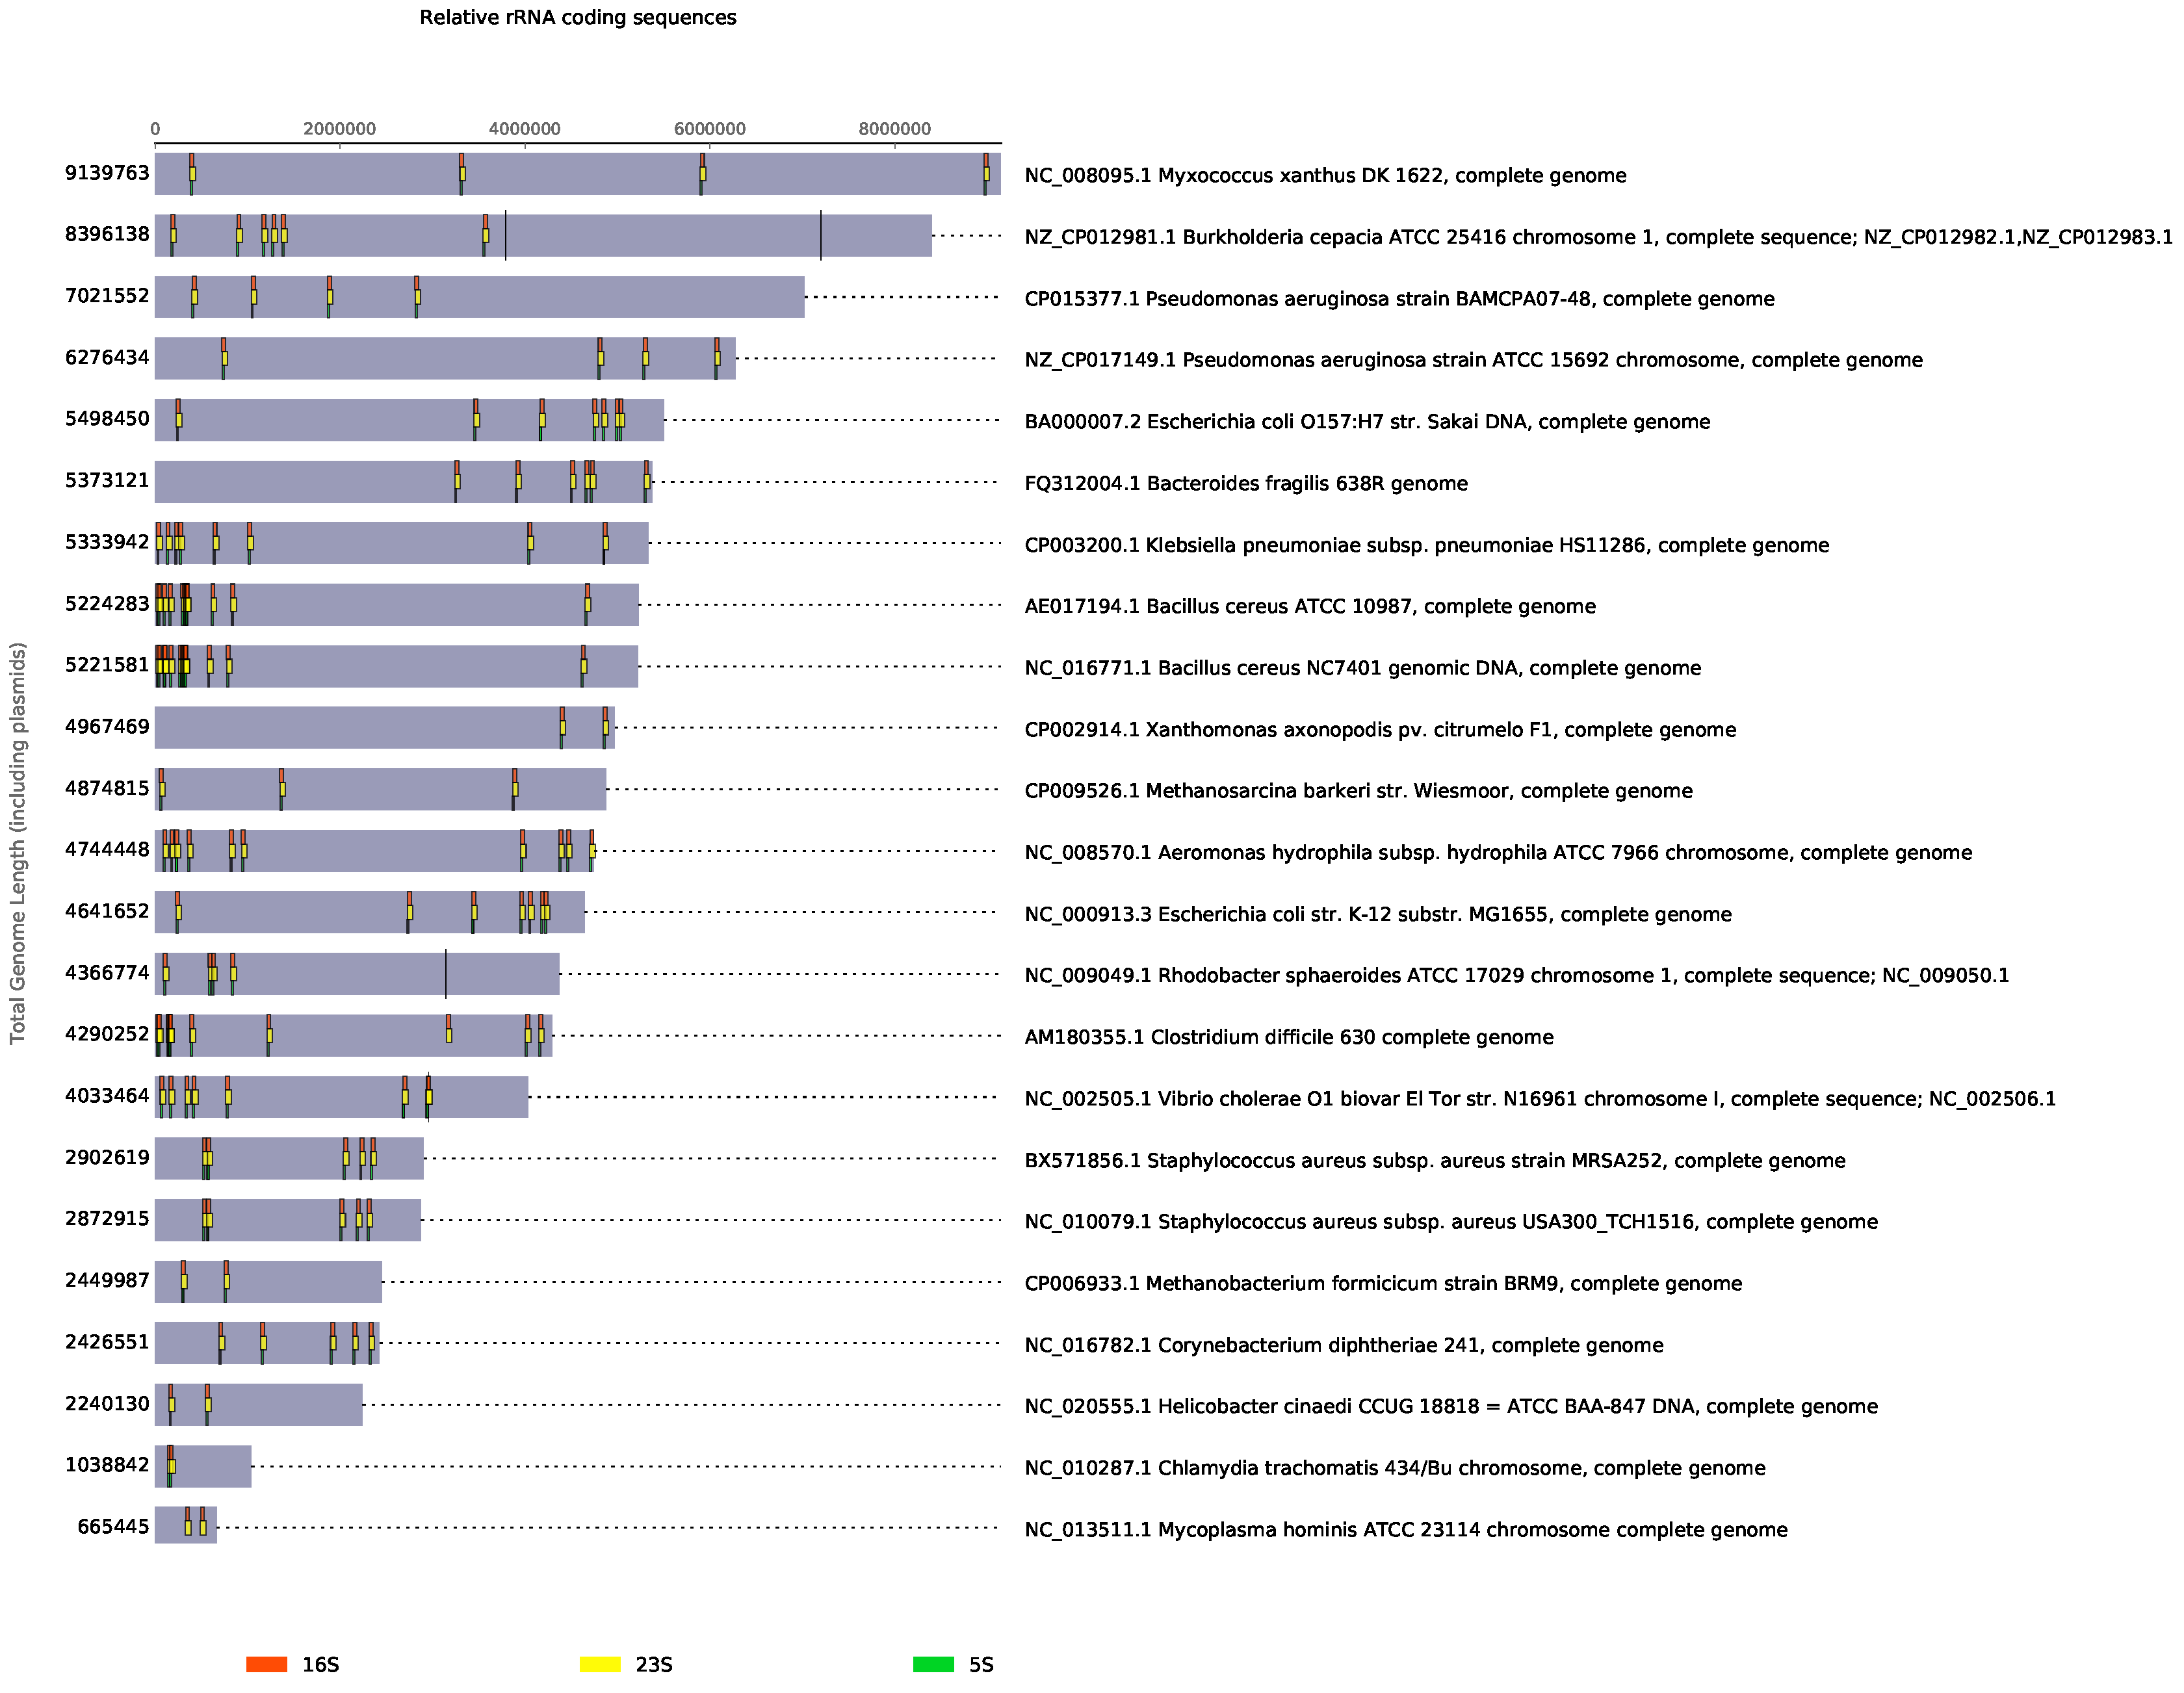
\includegraphics[width=1.0\textwidth]{normal_rDNA_relative_locations}
  \caption{Typical rDNA structure exhibited by strains used in this study.}
  \label{fig:typical}
\end{figure}

\section*{Key Parameters}
\subsection*{\texttt{--ref\_as\_contig}}
The assembly that results from including riboSeed's ``long reads'' is sensitive to the manner in which they are incorporated into the \textit{de novo} assembly. Here, for our analyses, we used the SPAdes assembler \cite{Bankevich2012}, as it has built-in ways to include contigs (using the ``--trusted-contigs'' or ``--untrusted-contigs'') in FASTA format.  Other assemblers could be used, but most require long reads to have a quality score associated with them, preventing direct use of riboSeed's long reads.

As mentioned in the Methods section, riboSeed uses the reference rDNA region in the initial subassembly;  in subsequent subassemblies, the longest contig of the previous subassembly is used.  These regions can be treated one of four ways using the \texttt{--ref\_as\_contig} argument: \texttt{trusted}, \texttt{untrusted}, \texttt{infer}, or \texttt{ignore}.  Additionally, if the user is worried that the reference rDNA will too heavily influence the initial subassembly, they can enable the \texttt{--initial\_consensus} flag to use a mapping consensus assembly instead of the de Bruijn graph based assembly from SPAdes.

The default manner in which rDNA regions (either from the reference or from the previous iteration's subassembly) behaviour is to infer (\texttt{--ref\_as\_contig infer}): if the percent of reads mapping to  the (whole) reference sequence  is over 80\%, than the rDNA region will be included as a trusted contig.  If below 80\%, the reads will be treated as untrusted.

If a user wishes to have the subassemblies only using the reads (true \textit{de novo} assembly), they can use the \texttt{ignore} option.  We only recommend this with very close references.

Further, if the user wishes to explicitly define the behaviour, \texttt{trusted} or \texttt{untrusted} can be provided to the \texttt{--ref\_as\_contig} argument.

\subsection*{\texttt{--score\_min}}
By default, the accepted alignment score for BWA mapping is $\frac{1}{2}$ the read length.  If needed, this can be increased for greater stringency when dealing with more divergent references, or decreased to include more reads, which may be advantageous when assembling a low coverage dataset.

% \section*{Excluding GAGE-B HiSeq \textit{B. cereus}}
\begin{figure}[H]
  \centering
  \begin{subfigure}[b]{.7\textwidth}
    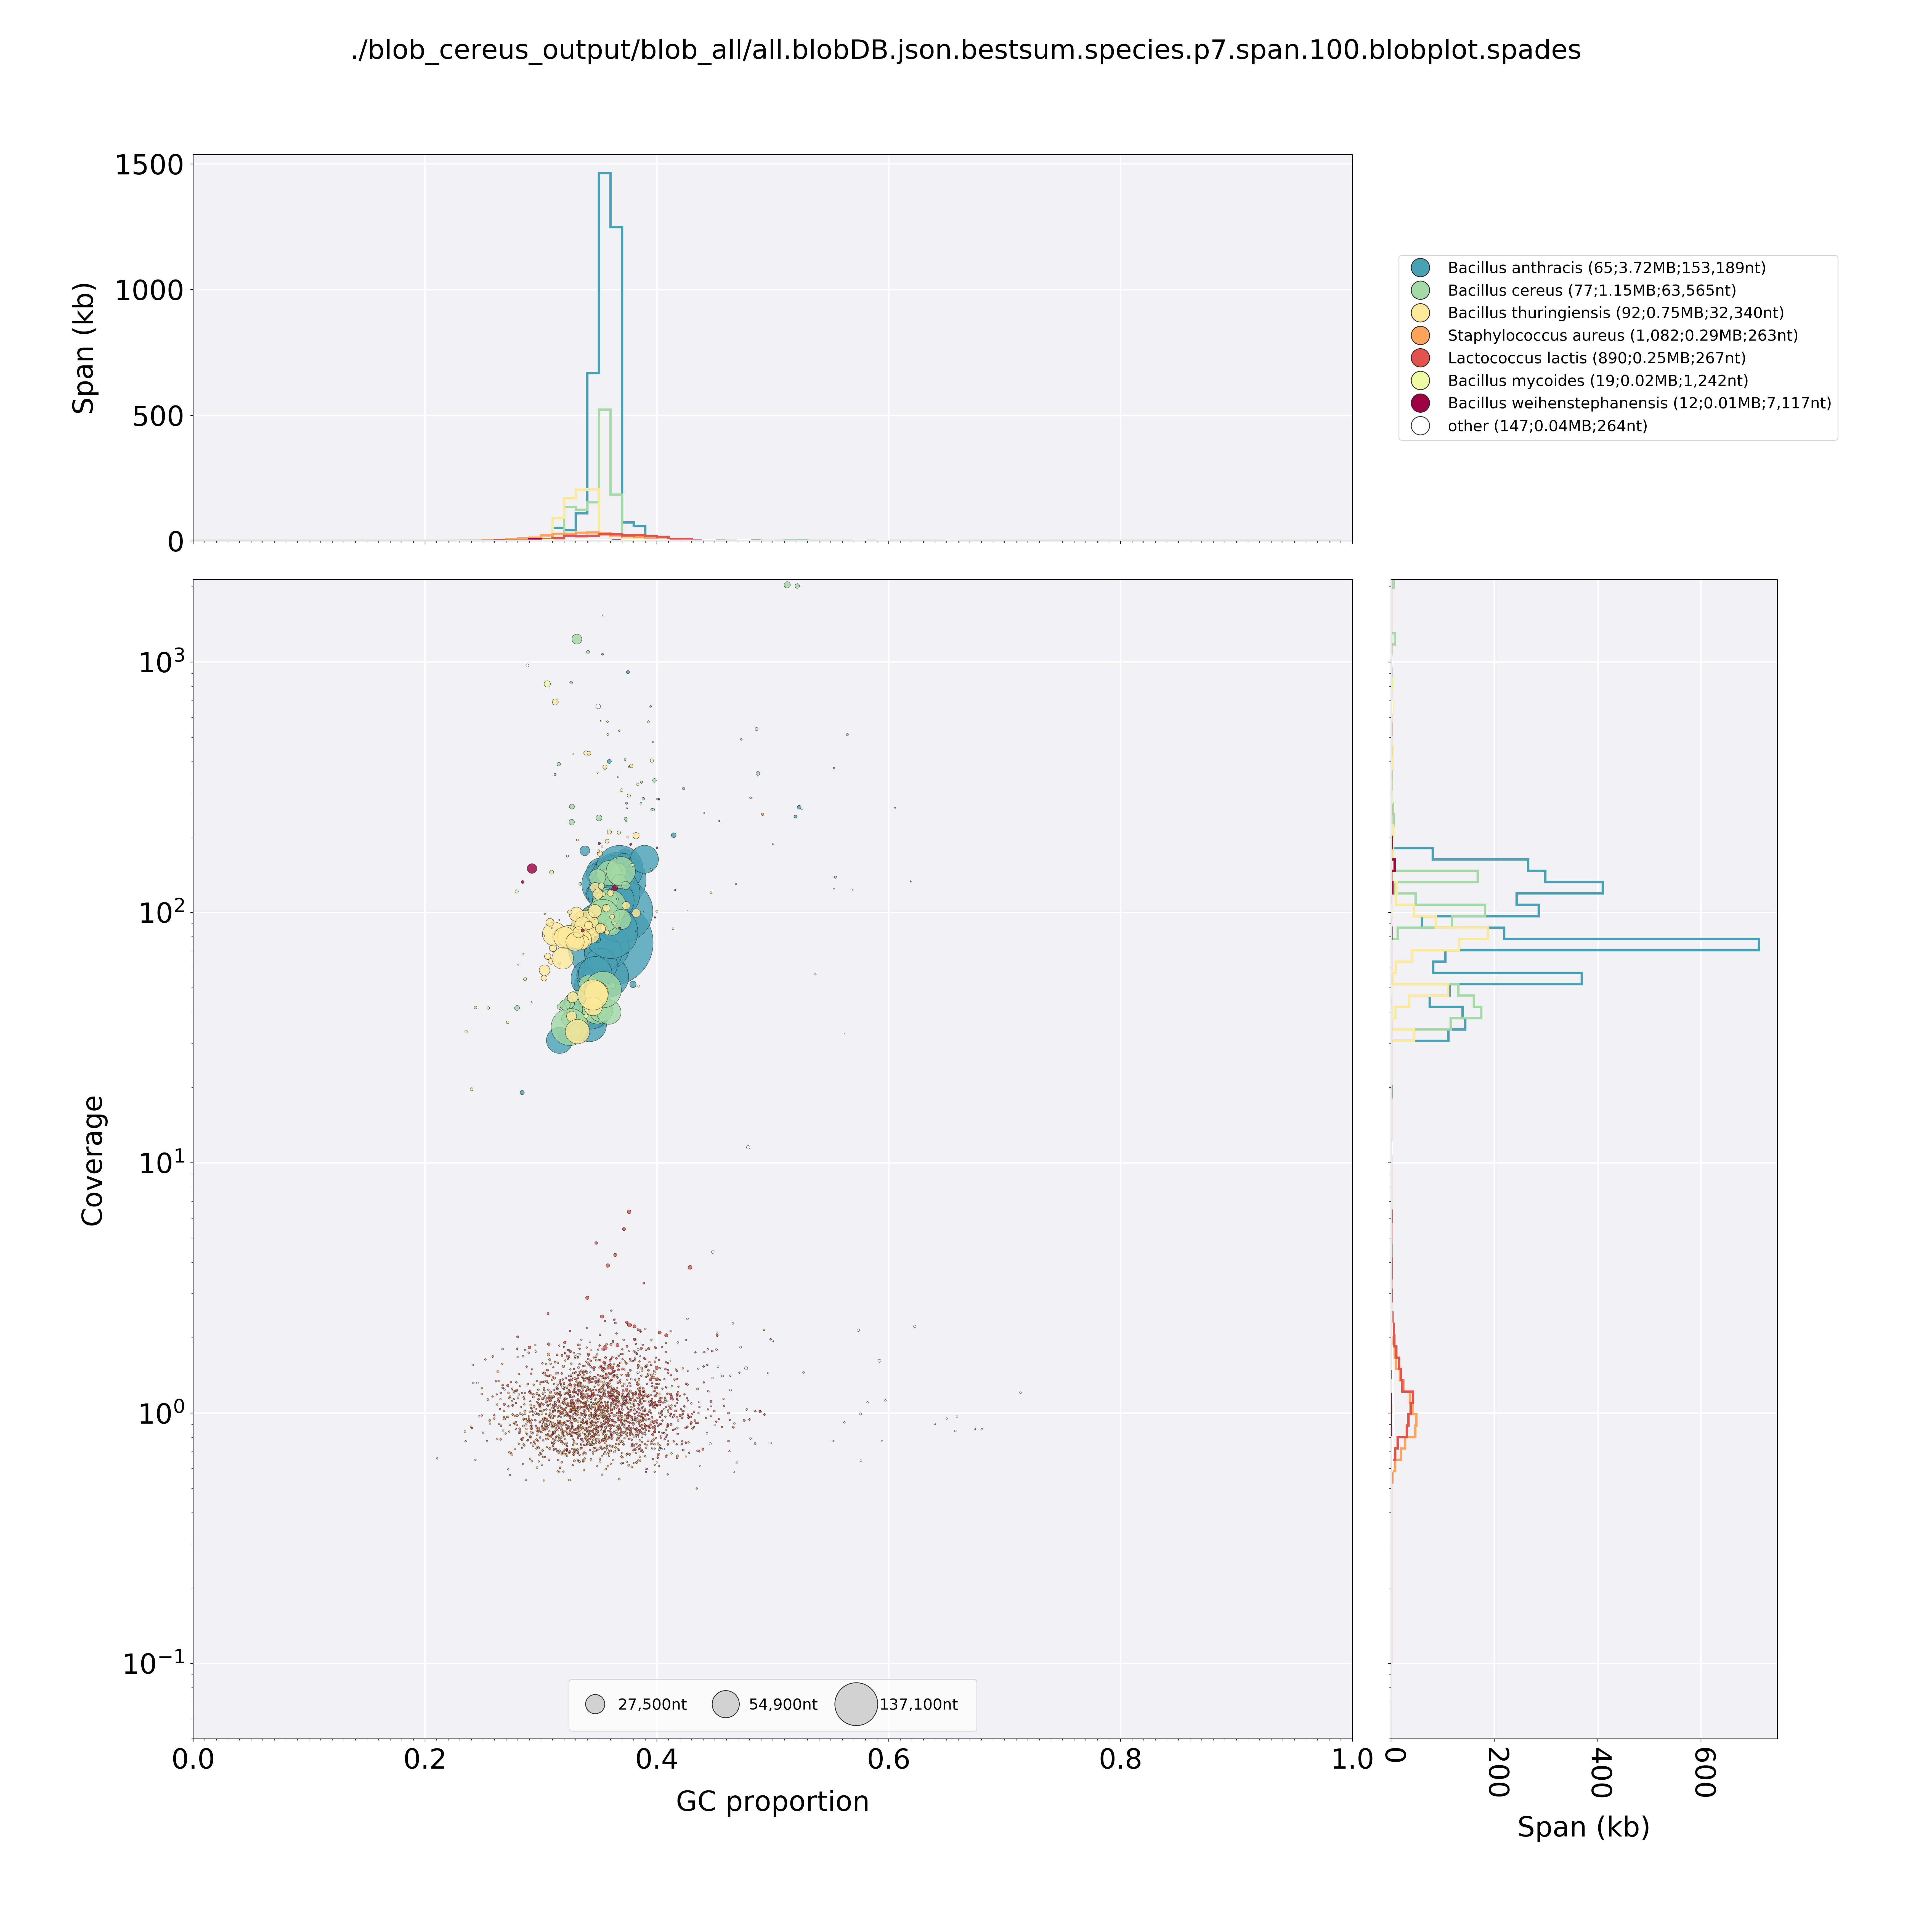
\includegraphics[width=.95\textwidth]{all.blobDB.json.bestsum.species.p7.span.100.blobplot.spades.png}
    \caption{All reads}
  \end{subfigure}
  \begin{subfigure}[b]{.7\textwidth}
    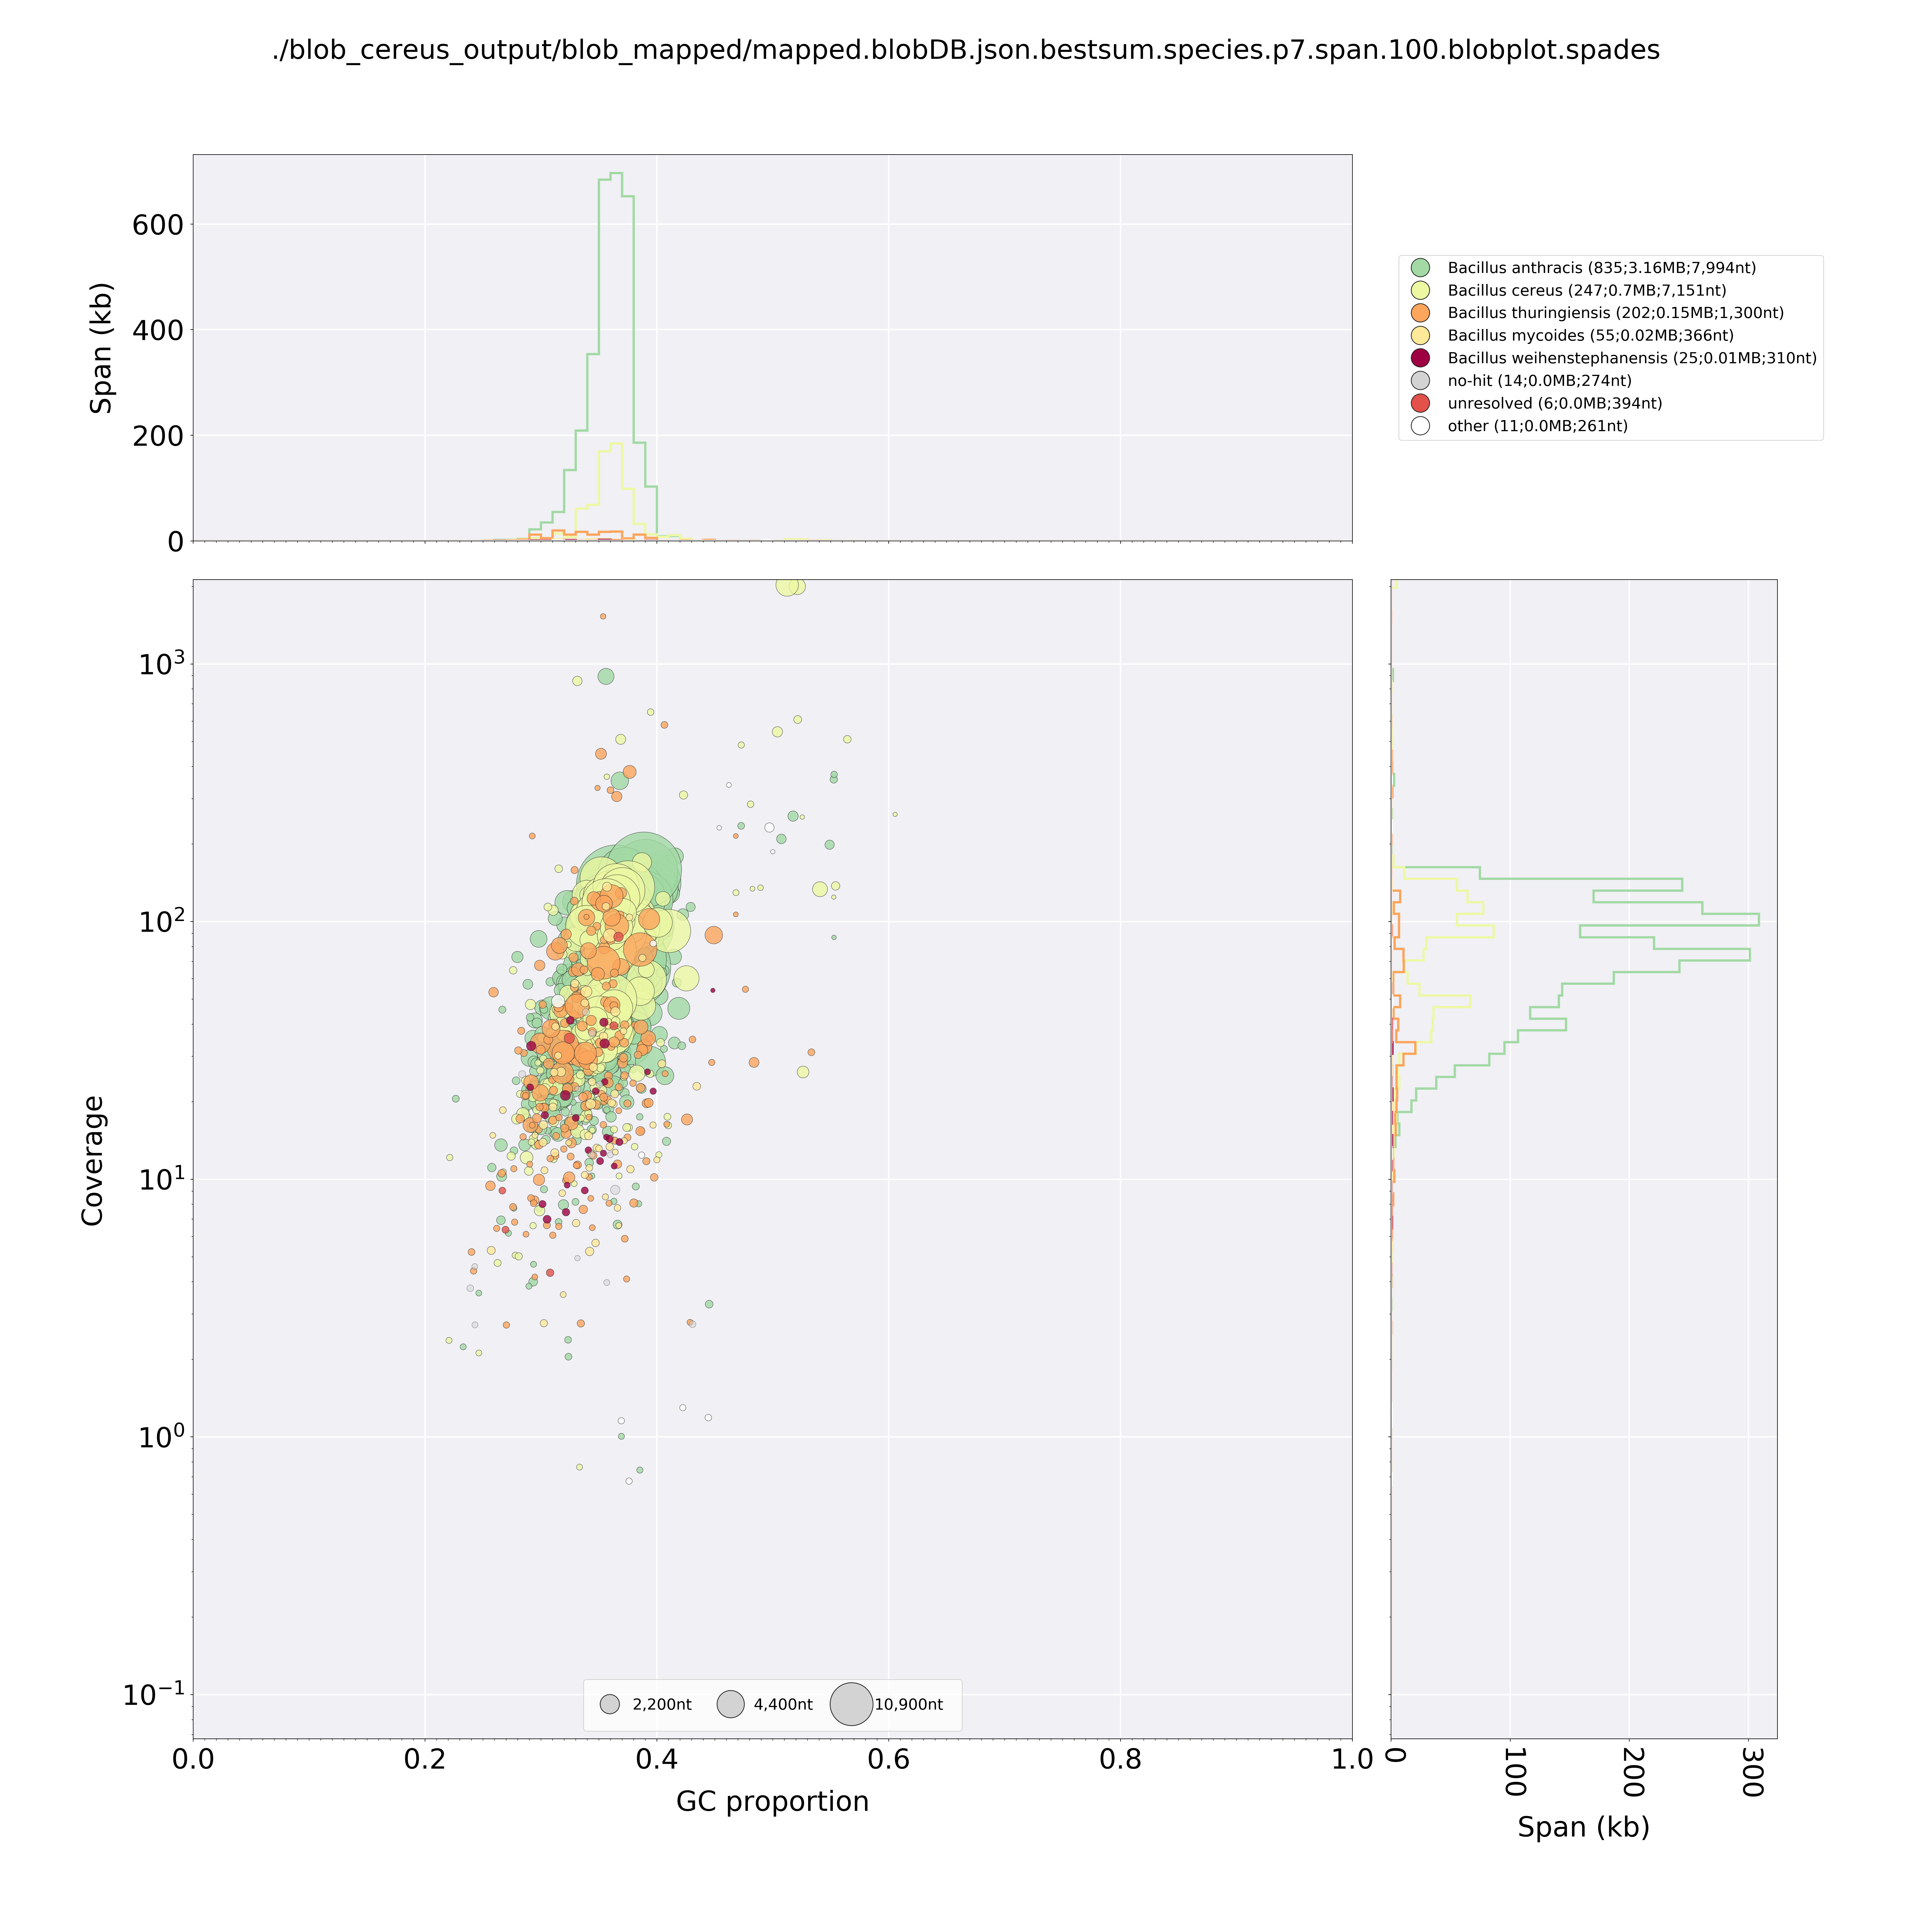
\includegraphics[width=.95\textwidth]{mapped.blobDB.json.bestsum.species.p7.span.100.blobplot.spades.png}
    \caption{Reads aligning to reference}
  \end{subfigure}
\end{figure}
\begin{figure}[H]\ContinuedFloat
  \centering
  \begin{subfigure}[b]{.7\textwidth}
    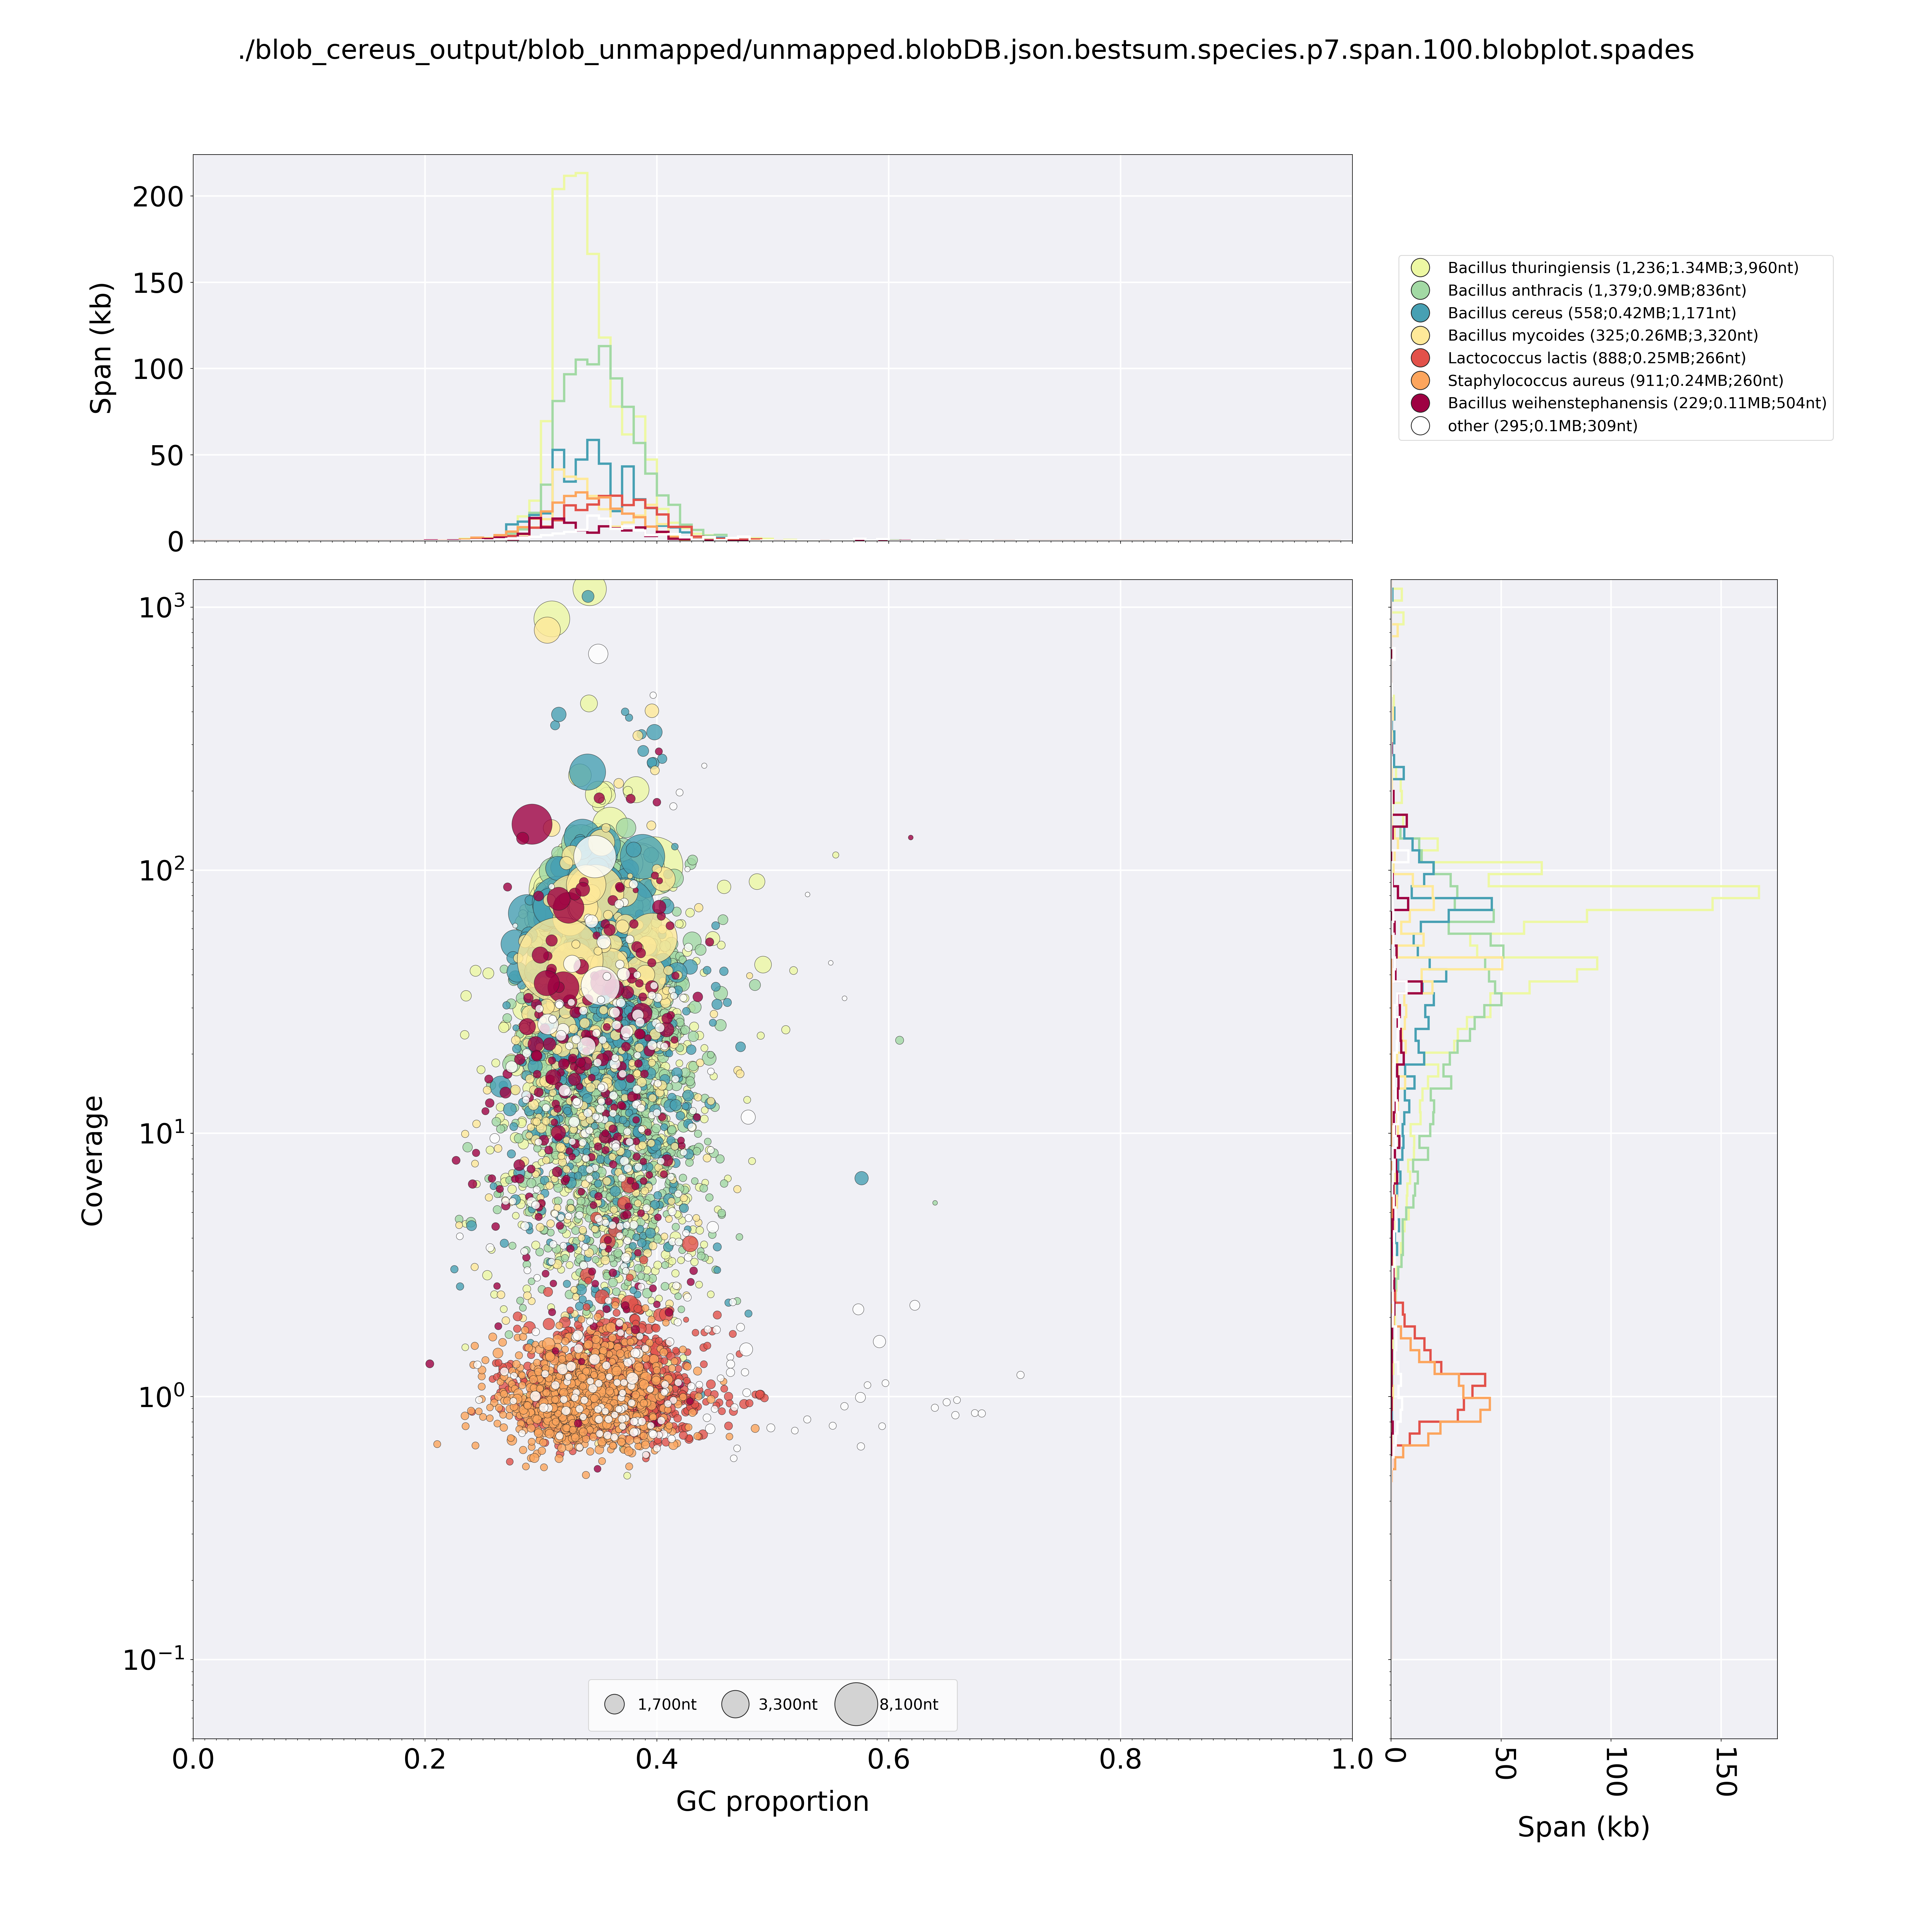
\includegraphics[width=.95\textwidth]{unmapped.blobDB.json.bestsum.species.p7.span.100.blobplot.spades.png}
    \caption{Reads failing to align to reference}
  \end{subfigure}
  \caption{Assessing contamination in the GAGE-B HiSeq \textit{B. cereus} dataset with blobtools. Reads were assembled with metaSPAdes, taxanomically assigned with BLASTn against the nt database, and plotted with blobtools.  (A) shows the whole dataset, while (B) and (C) shows the portion of the reads aligning to the \textit{B. cereus} ATCC 10987 reference and those failing to align, respectively.}
  \label{fig:contamination_all}
\end{figure}

The GAGE-B paper \cite{Magoc2013} notes that the \textit{B. cereus} HiSeq dataset proved particularly difficult to assemble. After noticing this irregularity, we re-assembled the trimmed reads downloaded from the GAGE-B website with metaSPAdes \cite{Nurk2017}  using default parameters.  Then, blastn was used to search the resulting contigs against NCBI's nt database (May, 2017) to get a list of hits according to the blobtools \cite{Laetsch2017a} specifications. Blobtools was then used to plot the hit coverage, taxonomy, and GC-content of the contigs.  This revealed what appears to be a contamination. \ref{fig:contamination_all}A. As the GC content of the contaminating organisms did not differ from \textit{B. cereus}, we believe that many tools that use GC-skew to detect contamination would not have detected the problem with this dataset.


To further show the contamination, we split reads into those read pairs mapping to the \textit{B. cereus} ATCC 10987 reference genome and those unmapped.  BWA MEM \cite{Li2013} was used to map the 12039737 reads to the reference genome;  samtools was used to separate the 7500534 reads (62\%) that mapped from the 3984200 reads (33\%) that failed to map with default parameters\footnote{The remaining \ttilde5 \% are those pairs where only one read aligned to the reference; these were ignored for this analysis.}.Each of these sets of reads was then assembled, BLASTed against the nt database, and plotted with blobtools \ref{fig:contamination_all}B and C.


Further, MaxBin \cite{Wu2014}, Kraken, and MBBC \cite{Wang2011} also supported the hypothesis that the sample is contaminated with approximately one third of reads originating from a non-\textit{B. cereus} strain.


\begin{table}[]
  \centering
  \caption{Hits resulting from searching the SRA database for various sequencing technologies as of January, 2017}
  \label{table:searchterms}
  \begin{tabular}{lrr}
    \toprule
    Search term & Hits & Percentage \\
    \midrule
    illumina & 2242225 & 94.27 \\
    pacbio & 21131 & 0.89 \\
    ion & 30560 & 1.28 \\
    roche & 42445 & 1.78 \\
    oxford & 12301 & 0.52 \\
    solid & 29791 & 1.25 \\
    \arrayrulecolor{lgray}\hline
    Total & 2378453 & 100\\
    \arrayrulecolor{black}
    \bottomrule
\end{tabular}
\end{table}

%%%%%%%%%%%%%%%%%%%%%%%%%%%%%%%%%%%%%%%%%%%%%%%%%%%%%%%%%%%%%%%%%%%%%%%
\begin{table}[!h]
\centering
\caption{Accessions for 25 \textit{E. coli} genomes used to calculate substitution rate}
\label{table:accessions}
\begin{tabular}{l}
  \toprule

  GCA\_000005845.2\_ASM584v2                    \\
  GCA\_000019385.1\_ASM1938v1                   \\
  GCA\_000026245.1\_ASM2624v1                   \\
  GCA\_000026345.1\_ASM2634v1                   \\
  GCA\_000026545.1\_ASM2654v1                   \\
  GCA\_000146735.1\_ASM14673v1                  \\
  GCA\_000257275.1\_ASM25727v1                  \\
  GCA\_000520055.1\_ASM52005v1                  \\
  GCA\_000732965.1\_ASM73296v1                  \\
  GCA\_001007915.1\_ASM100791v1                 \\
  GCA\_001442495.1\_ASM144249v1                 \\
  GCA\_001469815.1\_ASM146981v1                 \\
  GCA\_001660565.1\_ASM166056v1                 \\
  GCA\_001660585.1\_ASM166058v1                 \\
  GCA\_001753565.1\_ASM175356v1                 \\
  GCA\_001888075.1\_ASM188807v1                 \\
  GCA\_001901025.1\_ASM190102v1                 \\
  GCA\_001936315.1\_ASM193631v1                 \\
  GCA\_002056065.1\_ASM205606v1                 \\
  GCA\_002078295.1\_ASM207829v1                 \\
  GCA\_002156825.1\_ASM215682v1                 \\
  GCA\_002163935.1\_ASM216393v1                 \\
  GCA\_002192275.1\_ASM219227v1                 \\
  GCA\_002220265.1\_ASM222026v1                 \\
  GCA\_900096795.1\_Ecoli\_AG100\_Sample3\_Doxycycline\_Assembly \\
  \bottomrule
  {\tiny   All available at \texttt{ftp://ftp.ncbi.nlm.nih.gov/genomes/all/GCA/}}

\end{tabular}
\end{table}
%%%%%%%%%%%%%%%%%%%%%%%%%%%%%%%%%%%%%%%%%%%%%%%%%%%%%%%%%%%%%%%%%%%%%%%



\begin{table}[]
\centering
\caption{Strain names and accessions for reference genomes used in this study.For the full list, which includes strains used in the supplementary data, SRA accession numbers for reads, and more, please consult the supplementary file ``strain\_metadata.tab''}.
\label{table:strainlist}
\begin{tabular}{ll}
  \toprule
  Strain Name & Accession \\
  \midrule
  \textit{E. coli MG1655} & NC\_000913.3 \\
  \textit{E. coli Sakai} &  BA000007.2 \\
  \textit{A. hydrophila ATCC 7966} & NC\_008570.1 \\
  \textit{B. cereus ATCC 10987} & AE017194.1 \\
  \textit{B. cereus NC7401} & NC\_016771.1 \\
  \textit{B. fragilis 638R} & FQ312004.1 \\
  \textit{K. pneumoniae} & CP003200.1\\
  \textit{R. sphaeroides ATCC 17029} & NC\_009049.1, NC\_009050.1 \\
  \textit{S. aureus TCH1516} & NC\_010079.1 \\
  \textit{S. aureus MRSA252} & BX571856.1 \\
  \textit{V. cholerae El Tor str. N16961} & NC\_002505.1, NC\_002506.1 \\
  \textit{X. axonopodis pv. Citrumelo} & CP002914.1 \\
  \textit{P. aeruginosa BAMCPA07-48} & CP015377.1 \\
  \textit{P. aeruginosa ATCC 15692} & NZ\_CP017149.1\\
  \bottomrule
\end{tabular}
\end{table}

\begin{table}[]
  \centering
  \caption{Software Versions}
  \label{table:software}
  \begin{tabular}{ll}
    \toprule
    Tool & Version \\
    \midrule
    Mauve & 2015-02-13 build 0 \\
    BLAST+ & 2.2.28+ \\
    Barrnap & 0.8 \\
    BWA & 0.7.8-r455 \\
    samtools & 1.4.1 \\
    MAFFT & v7.310 \\
    SPAdes & v3.9.0 \\
    QUAST & 4.4 \\
    bedtools & 2.17.0 \\
    EMBOSS & 6.5.7 \\
    pIRS & 2.0.2\\
    seqtk & 1.2-r94\\
    Parsnp & v1.2 \\
    \bottomrule
  \end{tabular}
\end{table}

\begin{table}[]
\centering
\caption{QUAST \cite{Gurevich2013} results of \textit{P. aeruginosa} BAMCPA07-48 assemblies comparing \textit{de fere novo} assembly, \textit{de novo} assembly, and reference-based assembly (where the \textit{P. aeruginosa} ATCC 15692 reference is included in the \textit{de novo} assembly as a trusted contig).  Blue and red highlight the best and worst results, respectively.  riboSeed's \textit{de fere novo} assembly either outperforms or performs comparably to \textit{de novo} assembly in all categories.  Using the reference as a trusted contig results in longer assemblies but with a much higher rate of mismatches, indels, and misassemblies.}
\label{table:full_ref_compare}
\begin{tabular}{lrrr}
  & \textbf{\textit{de fere novo}} & \textbf{\textit{de novo}} & \textbf{reference-based} \\
Genome fraction (\%) & \cellcolor[HTML]{CDCDF9}98.106 & \cellcolor[HTML]{FBDADA}97.868 & 98 \\
Duplication ratio & 1.001 & 1.001 & \cellcolor[HTML]{FBDADA}1.017 \\
Largest alignment & 630503 & \cellcolor[HTML]{FBDADA}402463 & \cellcolor[HTML]{CDCDF9}757685 \\
Total aligned length & 6893293 & \cellcolor[HTML]{FBDADA}6876715 & \cellcolor[HTML]{CDCDF9}6993532 \\
NGA50 & 176510 & 176510 & \cellcolor[HTML]{FBDADA}135376 \\
LGA50 & \cellcolor[HTML]{CDCDF9}12 & 13 & \cellcolor[HTML]{FBDADA}14 \\
% \textbf{Misassemblies} &  &  &  \\
\# misassemblies & 2 & 2 & \cellcolor[HTML]{FBDADA}9 \\
Misassembled contigs length & 212498 & 212498 & \cellcolor[HTML]{FBDADA}2347560 \\
% \textbf{Mismatches} &  &  &  \\
\# mismatches per 100 kbp & 1.89 & \cellcolor[HTML]{CDCDF9}1.69 & \cellcolor[HTML]{FBDADA}11.66 \\
\# indels per 100 kbp & 2.48 & \cellcolor[HTML]{CDCDF9}2.44 & \cellcolor[HTML]{FBDADA}2.94 \\
\# N's per 100 kbp & 0 & 0 & 0 \\
% \textbf{Statistics without reference} &  &  &  \\
\# contigs & \cellcolor[HTML]{CDCDF9}154 & 159 & 388 \\
Largest contig & 630503 & \cellcolor[HTML]{FBDADA}402463 & \cellcolor[HTML]{CDCDF9}1103106 \\
Total length & 6893293 & \cellcolor[HTML]{FBDADA}6876715 & \cellcolor[HTML]{CDCDF9}7237564 \\
Total length (\textgreater= 1000 bp) & 6865091 & \cellcolor[HTML]{FBDADA}6848513 & \cellcolor[HTML]{CDCDF9}7130244 \\
Total length (\textgreater= 10000 bp) & \cellcolor[HTML]{CDCDF9}6687664 & 6663031 & \cellcolor[HTML]{FBDADA}6617370 \\
Total length (\textgreater= 50000 bp) & \cellcolor[HTML]{CDCDF9}6242010 & 6168232 & \cellcolor[HTML]{FBDADA}5534330
\end{tabular}
\end{table}


\begin{table}[ht]
\begin{center}
  \caption{Assembling \textit{S. aureus} UAMS-1 with BugBuilder. We did not have access to critical information about the pipeline parameters used in the original assembly; this prevented exact recapitulation of the published results. Therefore, we approximated the settings based on notes from the publication. The performance of Pilon \cite{Walker2014a}, GapFiller \cite{Boetzer2012}, or no finishing software was assessed with both the \textit{de fere novo} and \textit{de novo} assemblies. rDNA counts were visually determined using Mauve; all other metrics were generated with QUAST, using the scaffolds from the assemblies and the \textit{S. aureus} MRSA252 reference. Misassembly/mismatch stats were removed, as the reference and sequenced strain have an average nucleotide identity of 97.62\%, and the misassemblies cannot be differentiated from strain differences with QUAST. Blue and red highlight the best and worst results, respectively.}
\begin{tabular}{lrrr|rrr}

   & \multicolumn{3}{c}{\textbf{\textit{de fere novo}}} & \multicolumn{3}{c}{\textbf{\textit{de novo}}} \\
   & \textbf{GapFiller} & \textbf{Pilon} & \textbf{--} & \textbf{Gapfiller} &  \textbf{Pilon} & \textbf{--} \\
  rDNAs & \cellcolor[HTML]{CDCDF9}3 & \cellcolor[HTML]{CDCDF9}3 &\cellcolor[HTML]{CDCDF9} 3 & 0 & 0 & 0\\
  \# contigs ($\geq$ 0 bp) & 1 & 1 & 1 & 1 & 1 & 1 \\
  Total length & 2773352 & \cellcolor[HTML]{CDCDF9}2781986 & 2763179 & 2768273 & 2770267 & \cellcolor[HTML]{FBDADA}2752929 \\
  Reference length & 2902619 & 2902619 & 2902619 & 2902619 & 2902619 & 2902619 \\
  GC (\%) & 32.78 & 32.80 & 32.78 & 32.72 & 32.73 & 32.71 \\
  Reference GC (\%) & 32.81 & 32.81 & 32.81 & 32.81 & 32.81 & 32.81 \\
  Unaligned length & 20087 & \cellcolor[HTML]{CDCDF9}15391 & 19075 & 18980 & 16819 & \cellcolor[HTML]{FBDADA}20141 \\
  Genome fraction (\%) & 94.736 & \cellcolor[HTML]{CDCDF9}94.941 & 94.508 & 94.487 & 94.604 & \cellcolor[HTML]{FBDADA}94.105 \\
  Duplication ratio & 1.001 & 1.004 & \cellcolor[HTML]{CDCDF9}1.000 & 1.002 & 1.003 & \cellcolor[HTML]{CDCDF9}1.000 \\
  \# N's per 100 kbp & 151.44 & \cellcolor[HTML]{CDCDF9}58.59 & 160.65 & 184.23 & 111.00 & \cellcolor[HTML]{FBDADA}200.73 \\
  Largest alignment & 403935 & \cellcolor[HTML]{CDCDF9}469521 & \cellcolor[HTML]{FBDADA}403508 & 459120 & 459623 & \cellcolor[HTML]{FBDADA}403508 \\
  Total aligned length & 2753265 & \cellcolor[HTML]{CDCDF9}2766595 & 2744104 & 2749293 & 2753448 & \cellcolor[HTML]{FBDADA}2732788 \\
  NA50 & \cellcolor[HTML]{CDCDF9}223096 & 195659 & 222384 & 205820 & \cellcolor[HTML]{FBDADA}164646 & 222384 \\
  NGA50 & 176550 & 177158 & \cellcolor[HTML]{CDCDF9}222384 &\cellcolor[HTML]{FBDADA} 157488 & 164646 & 176039 \\
  LA50 & 5 & \cellcolor[HTML]{CDCDF9}5 & \cellcolor[HTML]{CDCDF9}5 & \cellcolor[HTML]{CDCDF9}5 & \cellcolor[HTML]{FBDADA}6 & \cellcolor[HTML]{CDCDF9}5 \\
  LGA50 & 6 & 6 & \cellcolor[HTML]{CDCDF9}5 & 6 & 6 & 6 \\
\end{tabular}
\end{center}
\end{table}


%%%%%%%%%%%%%%%%%%%%%%%%%%%%%%%%%%%%%%%%%%%%%%%%%%%%
\pagebreak
%%%%%%%%%%%%%%%%%%%%%%%%%%%%%%%%%%%%%%%%%%%%%%%%
\bibliographystyle{unsrt}
\bibliography{riboSeed_refs}

\end{document}
